% Szglab4
% ===========================================================================
%
\chapter{Szkeleton tervezése}

\thispagestyle{fancy}

\section{A szkeleton modell valóságos use-case-ei}
\comment{A szkeletonnak, mint önálló programnak a működésével kapcsolatos use-case-ek.}

\subsection{Use-case diagram}

\begin{figure}[h]
\begin{center}
%\includegraphics[width=17cm]{chapters/chapter05/example.pdf}
\caption{x}
\label{fig:SzkeletonUseCase}
\end{center}
\end{figure}

\subsection{Use-case leírások}
\comment{Minden use-case-hez külön}

\usecase{...}{...}{...}{...}

\section{A szkeleton kezelői felületének terve, dialógusok}
\comment{A szkeleton által elfogadott bemenetek , valamint a szöveges konzolon megjelenő kimenetek. A kiemenet formátuma olyan kell legyen, ami alapján a működés összevethető a korábbi szekvencia-diagramokkal.}

\section{Szekvencia diagramok a belső működésre}
\comment{A szkeletonban implementált szekvenciadiagramok. Tipikusan egy use-case egy diagram. Ezek megegyezhetnek a korábban specifikált diagramokkal, de az egyes életvonalakat (lifeline) egyértelműen a szkeletonban példányosított objektumokhoz kell tudni kötni. Azt kell megjeleníteni, hogy a szkeletonban létrehozott objektumok egymással hogyan fognak kommunikálni.}

\section{Kommunikációs diagramok}
%\comment{A szkeletonban, az egyes szkeleton-use-case-ek futása során létrehozott objektumok és kapcsolataik bemutatására szolgáló %diagramok. Ezek alapján valósítják meg a szkeleton fejlesztői az inicializáló kódrészleteket.}

\begin{figure}[H]
\begin{center}
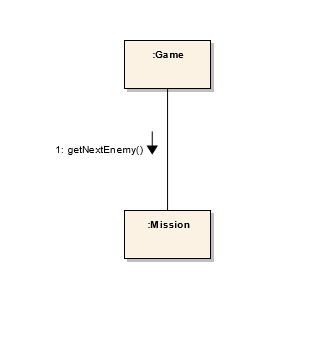
\includegraphics{images/ch05/nextEnemyKomm.png}
\caption{Ellenségek ütemezése.}
\label{fig:nextEnemyKomm}
\end{center}
\end{figure}

\begin{figure}[H]
\begin{center}
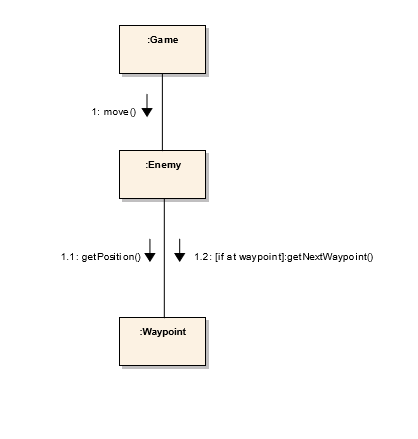
\includegraphics{images/ch05/moveKomm.png}
\caption{Ellenség mozgatása.}
\label{fig:moveKomm}
\end{center}
\end{figure}

\begin{figure}[H]
\begin{center}
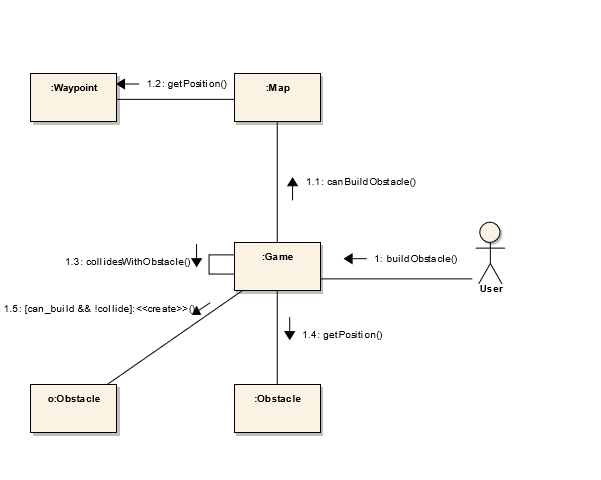
\includegraphics{images/ch05/buildObKomm.png}
\caption{Akadály építése.}
\label{fig:buildObKomm}
\end{center}
\end{figure}

\begin{figure}[H]
\begin{center}
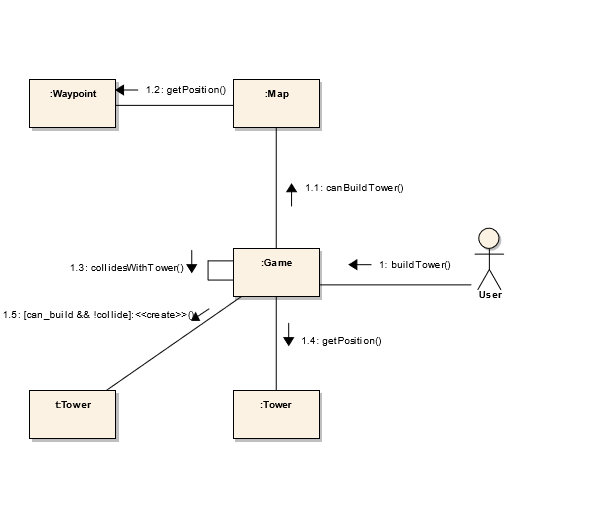
\includegraphics{images/ch05/buildTowerKomm.png}
\caption{Torony építése.}
\label{fig:buildTowerKomm}
\end{center}
\end{figure}

\begin{figure}[H]
\begin{center}
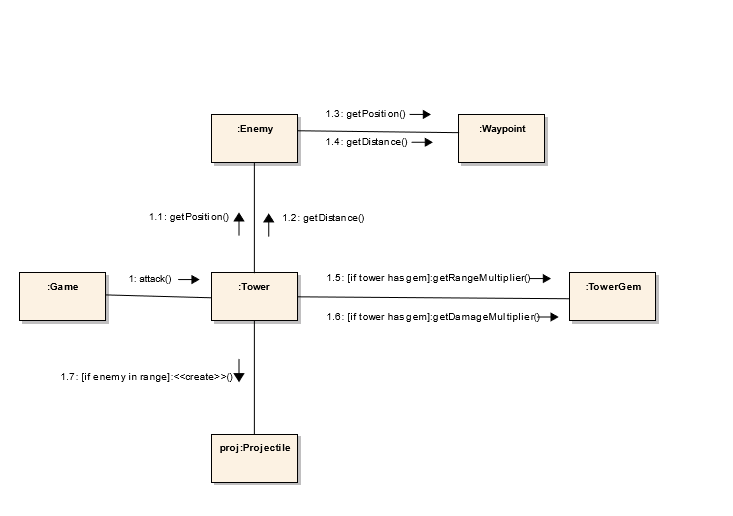
\includegraphics{images/ch05/attackKomm.png}
\caption{Torony tüzelése egy ellenségre.}
\label{fig:attackKomm}
\end{center}
\end{figure}

\begin{figure}[H]
\begin{center}
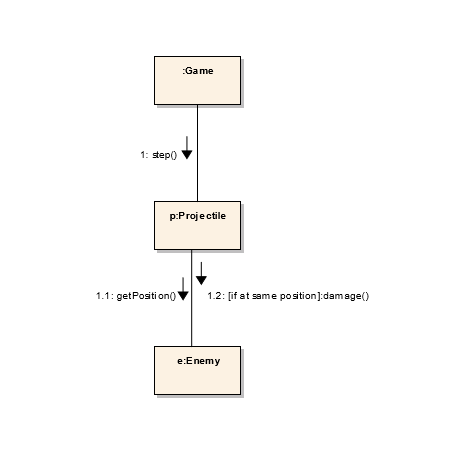
\includegraphics{images/ch05/projectileMoveKomm.png}
\caption{Lövedék mozgatása.}
\label{fig:projectileMoveKomm}
\end{center}
\end{figure}

\begin{figure}[H]
\begin{center}
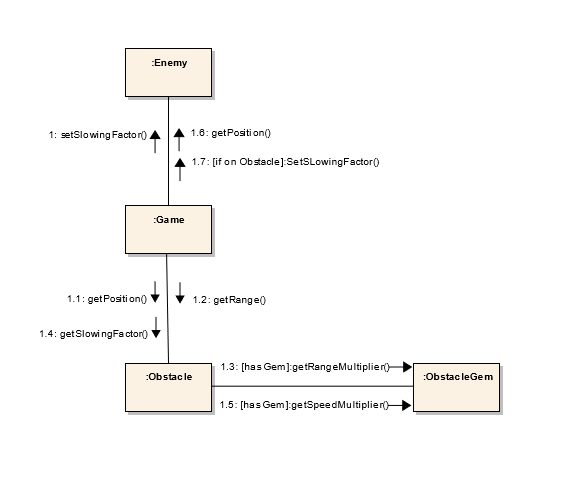
\includegraphics{images/ch05/slowKomm.png}
\caption{Akadályon áthaladó ellenség lassítása.}
\label{fig:slowKomm}
\end{center}
\end{figure}

\begin{figure}[H]
\begin{center}
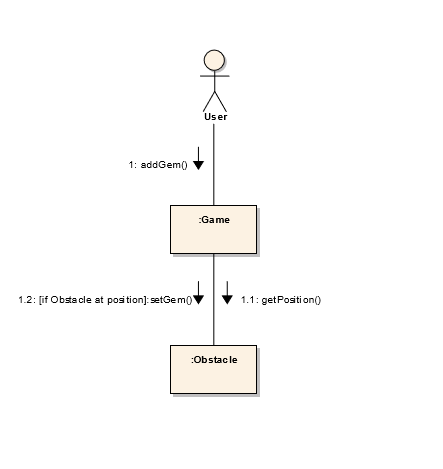
\includegraphics{images/ch05/addGemToObKomm.png}
\caption{Varázskő feltétele akadályra.}
\label{fig:addGemToObKomm}
\end{center}
\end{figure}


\begin{figure}[H]
\begin{center}
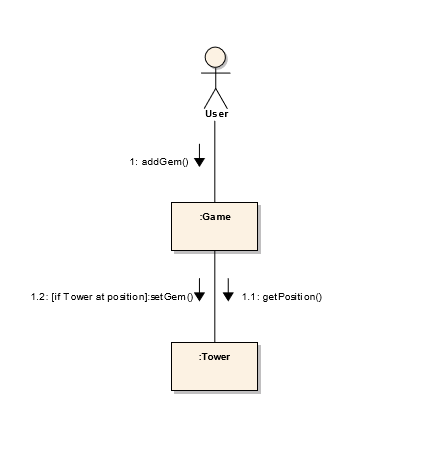
\includegraphics{images/ch05/addGemToTowerKomm.png}
\caption{Varázskő feltétele toronyra.}
\label{fig:addGemToTowerKomm}
\end{center}
\end{figure}